\documentclass{article}
\usepackage{graphicx} % Required for inserting images


% Set page size and margins
% Replace `letterpaper' with `a4paper' for UK/EU standard size
\usepackage[letterpaper,top=2cm,bottom=2cm,left=3cm,right=3cm,marginparwidth=1.75cm]{geometry}

% Useful packages
\usepackage{amsmath}
\usepackage{graphicx}
\usepackage[colorlinks=true, allcolors=blue]{hyperref}
\usepackage{listings}

\title{PS6 - ECON 5253}
\author{Hannah Bermudez}
\date{March 2025}

\begin{document}

\maketitle

\section{Introduction}
This document details the steps taken to clean and transform a dataset downloaded from Kaggle, analyze its structure, and visualize key relationships.

\section{Loading Required Packages}
To begin, I loaded the necessary R packages for data manipulation, visualization, and modeling:

\begin{lstlisting}[language=R, basicstyle=\ttfamily, keywordstyle=\color{blue}]
library(reticulate)
library(tidyverse)
library(ggplot2)
library(modelsummary)
library(broom)
\end{lstlisting}

\section{Installing and Setting Up Kaggle API}
The Kaggle API was installed using the following command in the command prompt:

\begin{lstlisting}[language=bash]
python -m pip install kaggle
\end{lstlisting}

In R, I ensured the API was available and set the API key:

\begin{lstlisting}[language=R]
reticulate::py_require("kaggle")
Sys.setenv(KAGGLE_CONFIG_DIR = "C:/Users/berm0006/Downloads/")
\end{lstlisting}

\section{Downloading the Dataset}
The dataset was downloaded from Kaggle and extracted:

\begin{lstlisting}[language=Python]
import kaggle
kaggle.api.dataset_download_files('deadier/play-games-and-success-in-
students', path='C:/Users/berm0006/Downloads/', unzip=True)
\end{lstlisting}

\section{Loading and Exploring the Data}
The dataset was then loaded into R:

\begin{lstlisting}[language=R]
game <- read.csv("C:/Users/berm0006/Downloads/gameandgrade.csv")
head(game)
\end{lstlisting}

\section{Data Cleaning}
I removed any rows that contained missing values:

\begin{lstlisting}[language=R]
game <- na.omit(game)
\end{lstlisting}

I also eliminated a data misclassification with the Playing.Games variable:

\begin{lstlisting}[language=R]
game <- game[game$Playing.Games %in% c(0, 1), ]
\end{lstlisting}

Finally, the Grade variable was converted to numeric format in order to properly use it:

\begin{lstlisting}[language=R]
game$Grade <- as.numeric(game$Grade)
\end{lstlisting}

\section{Data Visualizations}

\subsection{Visualization - 1}

\begin{figure}[h]
    \centering
    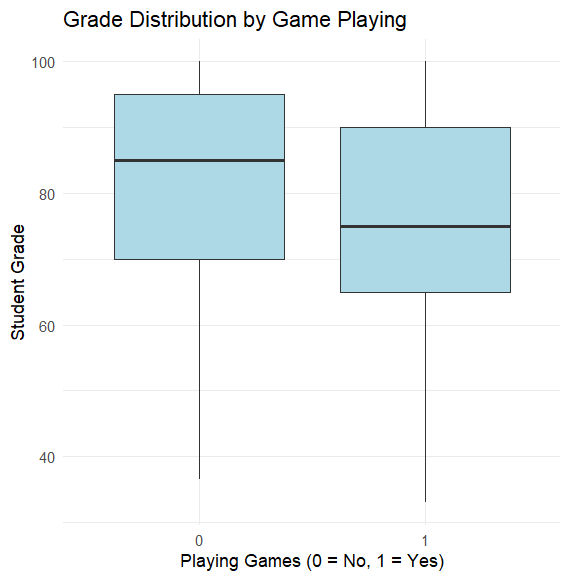
\includegraphics[width=0.7\textwidth]{PS6a_Bermudez.png}
    \caption{Boxplot of Grade Distribution by Game Playing}
    \label{fig:grade_distribution1}
\end{figure}

\begin{itemize}
    \item The median grade is higher for non-gamers than for gamers.
    \item The whiskers suggest that both groups have a wide spread of grades, but gamers have a lower median.
    \item There are no extreme outliers present.
\end{itemize}

Interpretation: Students who do not play games tend to have slightly higher grades on average compared to those who do play games.

\vspace{20pt}

\subsection{Visualization - 2}

\begin{figure}[h]
    \centering
    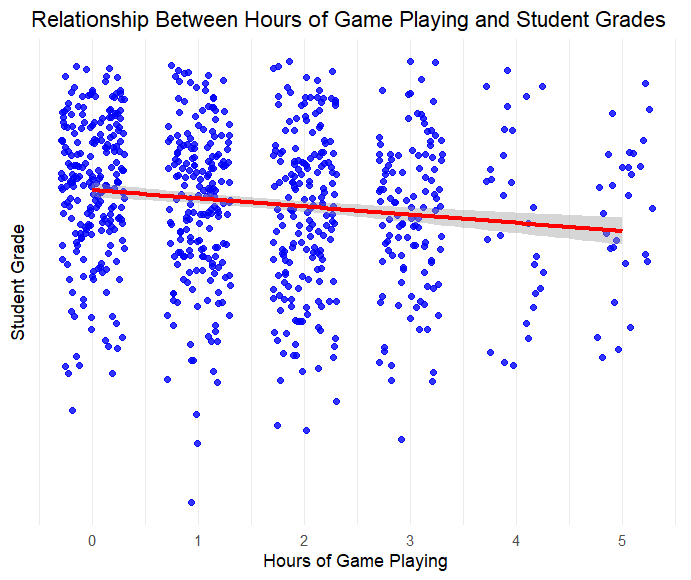
\includegraphics[width=0.7\textwidth]{PS6b_Bermudez.png}
    \caption{Scatterplot with Regression Line}
    \label{fig:grade_distribution2}
\end{figure}

\begin{itemize}
    \item The red regression line with a shaded confidence interval shows a slight negative trend, suggesting that as hours of game playing increase, student grades tend to decrease.
    \item The data points are widely spread, indicating high variability in student performance regardless of gaming hours.
    \item The negative slope of the regression line suggests that increased gaming hours may be associated with lower grades, but the effect appears relatively small.
\end{itemize}

Interpretation: There is a negative relationship between the number of hours spent playing games and student grades, meaning that an increase in hours played will lead to a decrease in student grades.

\vspace{4in}

\subsection{Visualization - 3}

\begin{figure}[h]
    \centering
    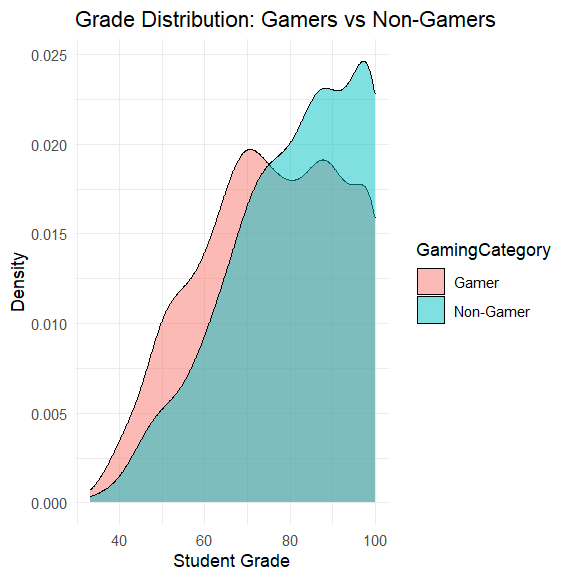
\includegraphics[width=0.7\textwidth]{PS6c_Bermudez.png}
    \caption{Density Plot of Grade Distribution}
    \label{fig:grade_distribution3}
\end{figure}

\begin{itemize}
    \item Non-gamers have a higher concentration of grades near the upper end (closer to 100), indicating that they tend to achieve higher grades overall.
    \item Gamers show a broader distribution, with a peak around the mid-range but fewer high-performing students compared to non-gamers.
    \item The overlapping areas suggest that while some gamers achieve high grades, non-gamers are more likely to perform better academically on average.
\end{itemize}

Interpretation: Non-gamers generally tend to have higher grades, whereas gamers exhibit more variability in academic performance, with a greater presence in the lower and mid-range grade categories.

\end{document}
